\documentclass[border=4pt]{standalone}
\usepackage{fontspec}
\usepackage{amsmath}
\usepackage{unicode-math}
\setmainfont{Latin Modern Roman}
\setmathfont{Latin Modern Math}
\usepackage{pgfplots}
\usepackage{pgfplotstable}
\pgfplotsset{compat=1.18}
\usepackage{tkz-euclide}
\usetikzlibrary{arrows.meta,calc,angles,quotes,patterns,3d,backgrounds}
\definecolor{ink}{HTML}{123428}
\definecolor{asy}{HTML}{475569}
\definecolor{mint}{HTML}{86e0bd}
\tikzset{asym/.style={asy, line width=0.9pt, dash pattern=on 5pt off 3.5pt},
         guide/.style={gray!70, line width=0.6pt, densely dotted},
         dot/.style={circle, inner sep=0pt, minimum size=5pt, draw=white, line width=0.5pt},
         odot/.style={circle, inner sep=0pt, minimum size=5.5pt, fill=white, line width=1pt},
         lab/.style={font=\footnotesize, inner sep=1.5pt, text=ink}}
\begin{document}
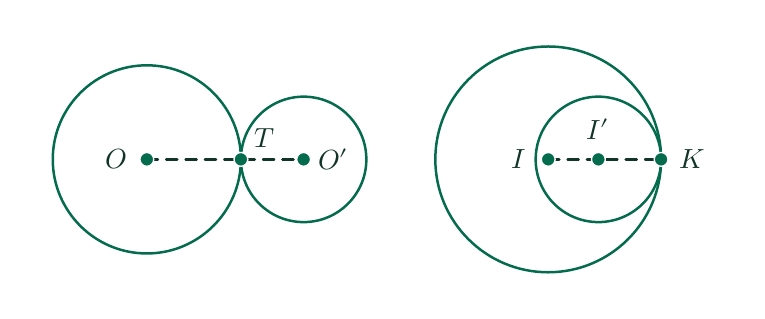
\begin{tikzpicture}[x=0.7965cm, y=0.7965cm]
\tkzDefPoint(0,0){O}
\tkzDefPoint(2.5,0){O1}
\tkzDefPoint(1.5,0){T}
\tkzDefPoint(1.5,0){tmp1}
\tkzDefPoint(3.5,0){tmp2}
\tkzDefPoint(6.4,0){I}
\tkzDefPoint(7.2,0){I1}
\tkzDefPoint(8.2,0){K}
\tkzDefPoint(8.2,0){tmp3}
\tkzDefPoint(8.2,0){tmp4}
\begin{scope}
\clip (-1.9,-2.1) rectangle (9.4,2.1);
\tkzDrawCircle[draw={rgb,255:red,4;green,107;blue,77}, line width=0.9pt](O,tmp1)
\tkzDrawCircle[draw={rgb,255:red,4;green,107;blue,77}, line width=0.9pt](O1,tmp2)
\tkzDrawCircle[draw={rgb,255:red,4;green,107;blue,77}, line width=0.9pt](I,tmp3)
\tkzDrawCircle[draw={rgb,255:red,4;green,107;blue,77}, line width=0.9pt](I1,tmp4)
\tkzDrawSegment[draw=ink, line width=0.90pt, dash pattern=on 4pt off 3pt](O,O1)
\tkzDrawSegment[draw=ink, line width=0.90pt, dash pattern=on 4pt off 3pt](I,K)
\end{scope}
\node[dot, fill={rgb,255:red,4;green,107;blue,77}] at (O) {};
\node[dot, fill={rgb,255:red,4;green,107;blue,77}] at (O1) {};
\node[dot, fill={rgb,255:red,4;green,107;blue,77}] at (T) {};
\node[dot, fill={rgb,255:red,4;green,107;blue,77}] at (I) {};
\node[dot, fill={rgb,255:red,4;green,107;blue,77}] at (I1) {};
\node[dot, fill={rgb,255:red,4;green,107;blue,77}] at (K) {};
\node[lab, font=\normalsize, anchor=center, xshift=-11pt, yshift=0pt] at (0,0) {$O$};
\node[lab, font=\normalsize, anchor=center, xshift=11pt, yshift=0pt] at (2.5,0) {$O'$};
\node[lab, font=\normalsize, anchor=center, xshift=7.78pt, yshift=7.78pt] at (1.5,0) {$T$};
\node[lab, font=\normalsize, anchor=center, xshift=-11pt, yshift=0pt] at (6.4,0) {$I$};
\node[lab, font=\normalsize, anchor=center, xshift=0pt, yshift=11pt] at (7.2,0) {$I'$};
\node[lab, font=\normalsize, anchor=center, xshift=11pt, yshift=0pt] at (8.2,0) {$K$};
\end{tikzpicture}
\end{document}
